\documentclass[amsmath,amssymb,notitlepage,12pt]{revtex4-1}
\usepackage{graphicx}
\usepackage{bm}% bold math
\usepackage{multirow}
\usepackage{booktabs}
\usepackage{verbatim}
\usepackage{hyperref}
\hypersetup{pdftex,colorlinks=true,allcolors=blue}
\usepackage{hypcap}
%\usepackage[small,compact]{titlesec}
%\usepackage{showkeys}
%\addtolength{\textheight}{0.3cm}
%\addtolength{\topmargin}{-0.15cm}
%\addtolength{\textwidth}{0.4cm}
%\addtolength{\hoffset}{-0.2cm}
\begin{document}
%\hspace*{11.5cm}CLAS-NOTE 2013-008

\title{HPS ECal Pedestals in the 2014 Commissioning Run}%\\Version 0.1}
\author{N. Baltzell}
\affiliation{Jefferson Lab}
\date{\today}
%\begin{abstract}
%\end{abstract}
\maketitle
%\tableofcontents

%\section{Introduction}
%No significant time-dependence of pedestals exists in the 2014 commissioning run.
%There is a clear rate-dependence of the pedestals due to pileup that can be addressed in offline analysis and in the trigger for the next run.  With 200 nA beam on 5 um Pt, the average effect for channels close to the beam is a 4 ADC decrease in the pedstals.  In a few extreme channels, it should result in a 60 MeV understimate of the pulse energy with our current pedestal subtraction.
\section{Pedestal Measurement}

\subsection{Mode 1}
In the FADC mode-1 data in this study, all samples in a 400 ns time window were readout with no threshold requirement.  In the case of cosmic trigger, the pedestals were taken from regions of that time window far from the cosmic signal.  In the case of only a random pulser trigger, all samples within the window were used.  In both cases the pedestal was calculated as the mean ADC value.  The difference between these pedestals before and after the 2014 commissioning run is small, shown in Figure \ref{fig:ped_3464-2915}. 

\begin{figure}[htbp]\centering
    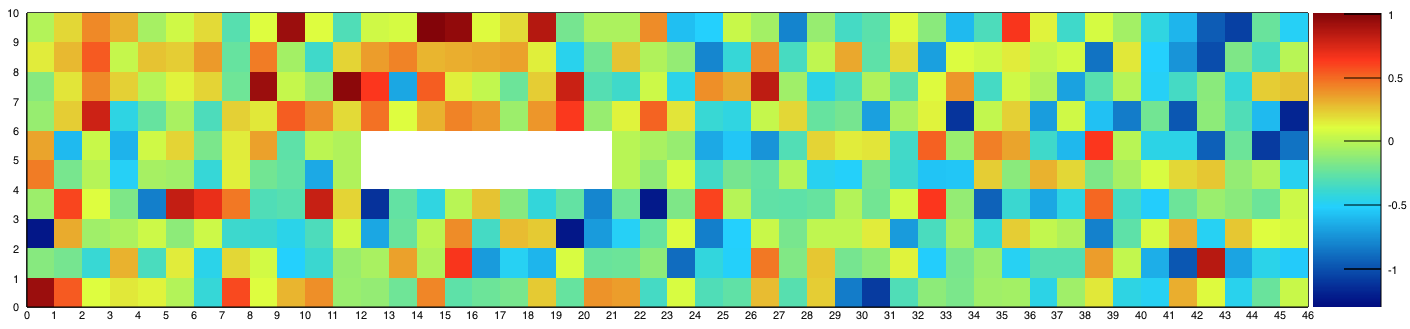
\includegraphics[width=17cm]{pics/ped_3464-2915.png}
    \caption{The difference between the pedestals calculated from dedicated FADC mode-1 runs before (run 2915) and after (run 3464) the commissioning run.  The majority of channels changed by less than 0.5 ADC, and none by more than 1 ADC.\label{fig:ped_3464-2915}}
\end{figure}

\subsection{Mode 7}
For the FADC mode-7 data in this study, an event-by-event ``pedestal'' was recorded directly in the data stream from the average of the first four samples in the time window.  The trigger for readout was on the calorimeter with a threshold of 12 ADC, and our physics signal is well separated in time from those first four samples by design of the readout window. 
%Readout windows that registered a pulse near the beginning of the time window were rejected in this caluculation (this can be a source of bias).
That event-by-event pedestal was then averaged over many events offline, and a gaussian fit of the resulting distribution did not give different result.  The run-dependence of the pedestals is shown in Figure \ref{fig:pedvsrun}.

\begin{figure}[htbp]\centering
    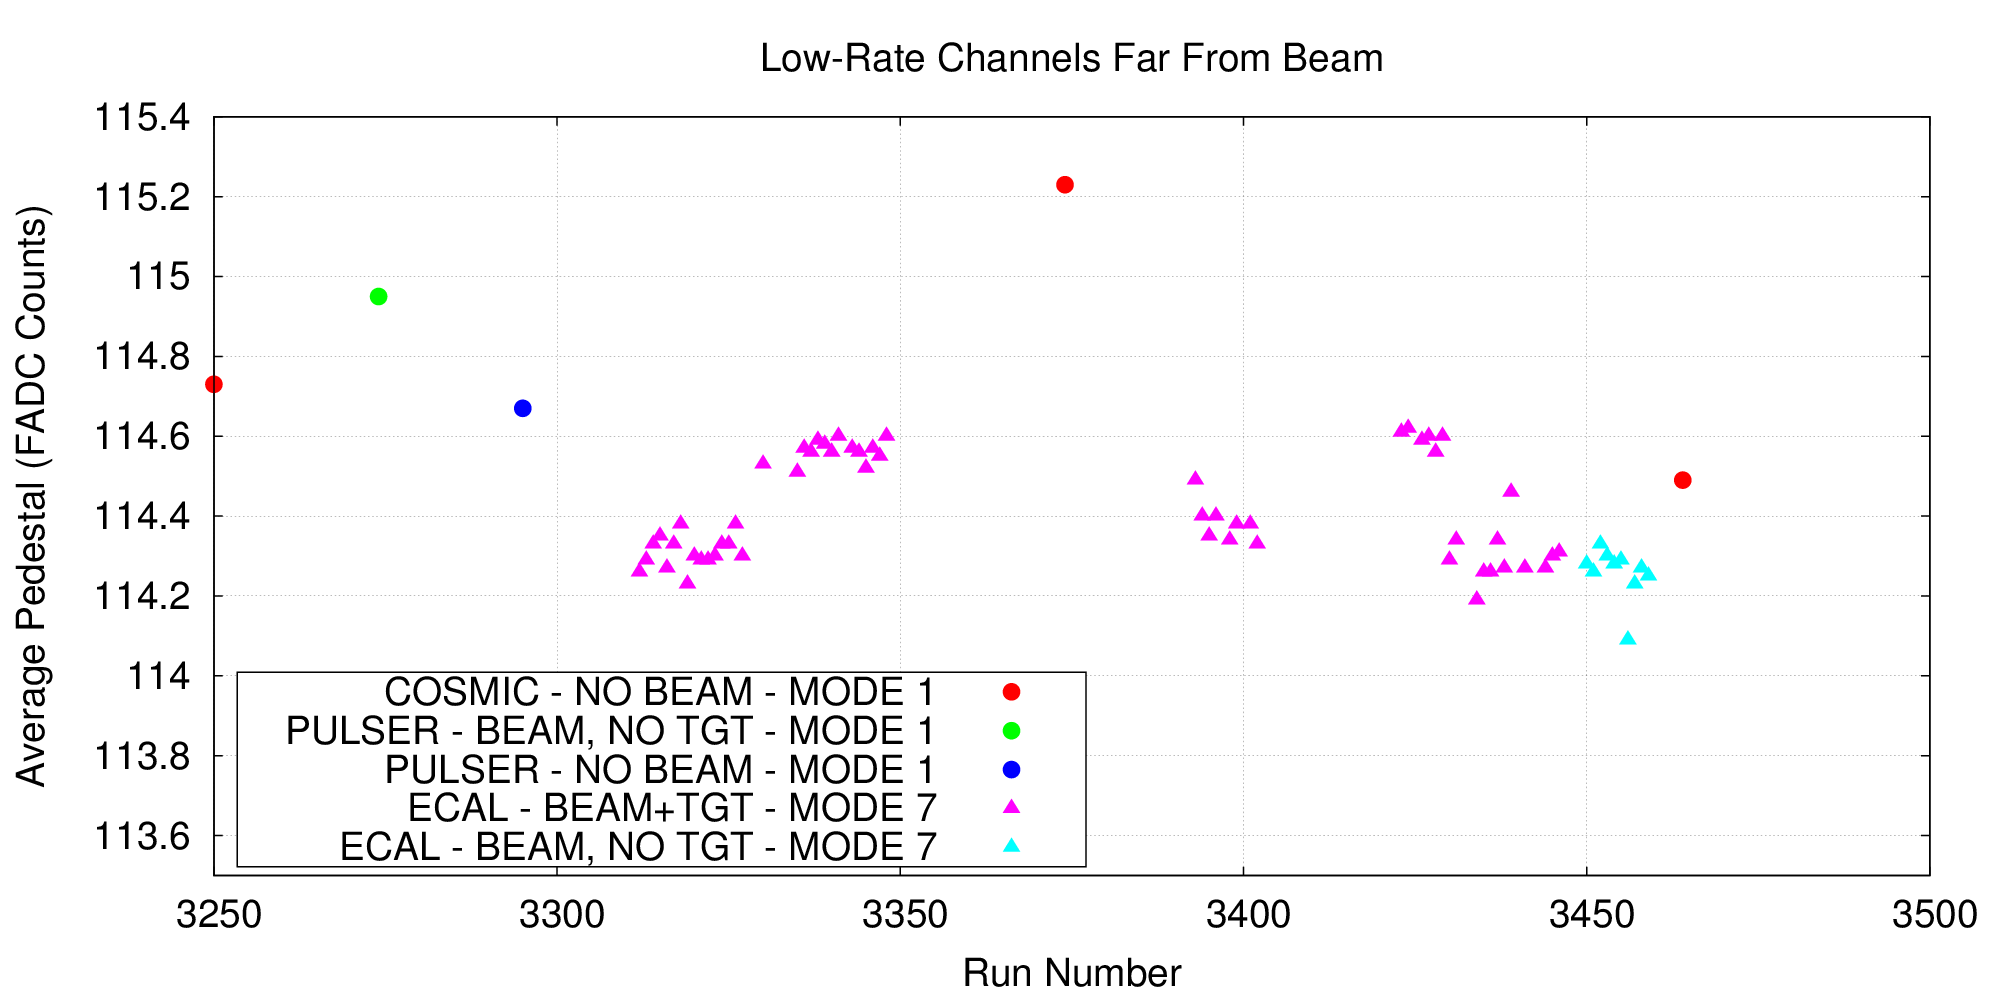
\includegraphics[width=14cm]{pics/low.png}
    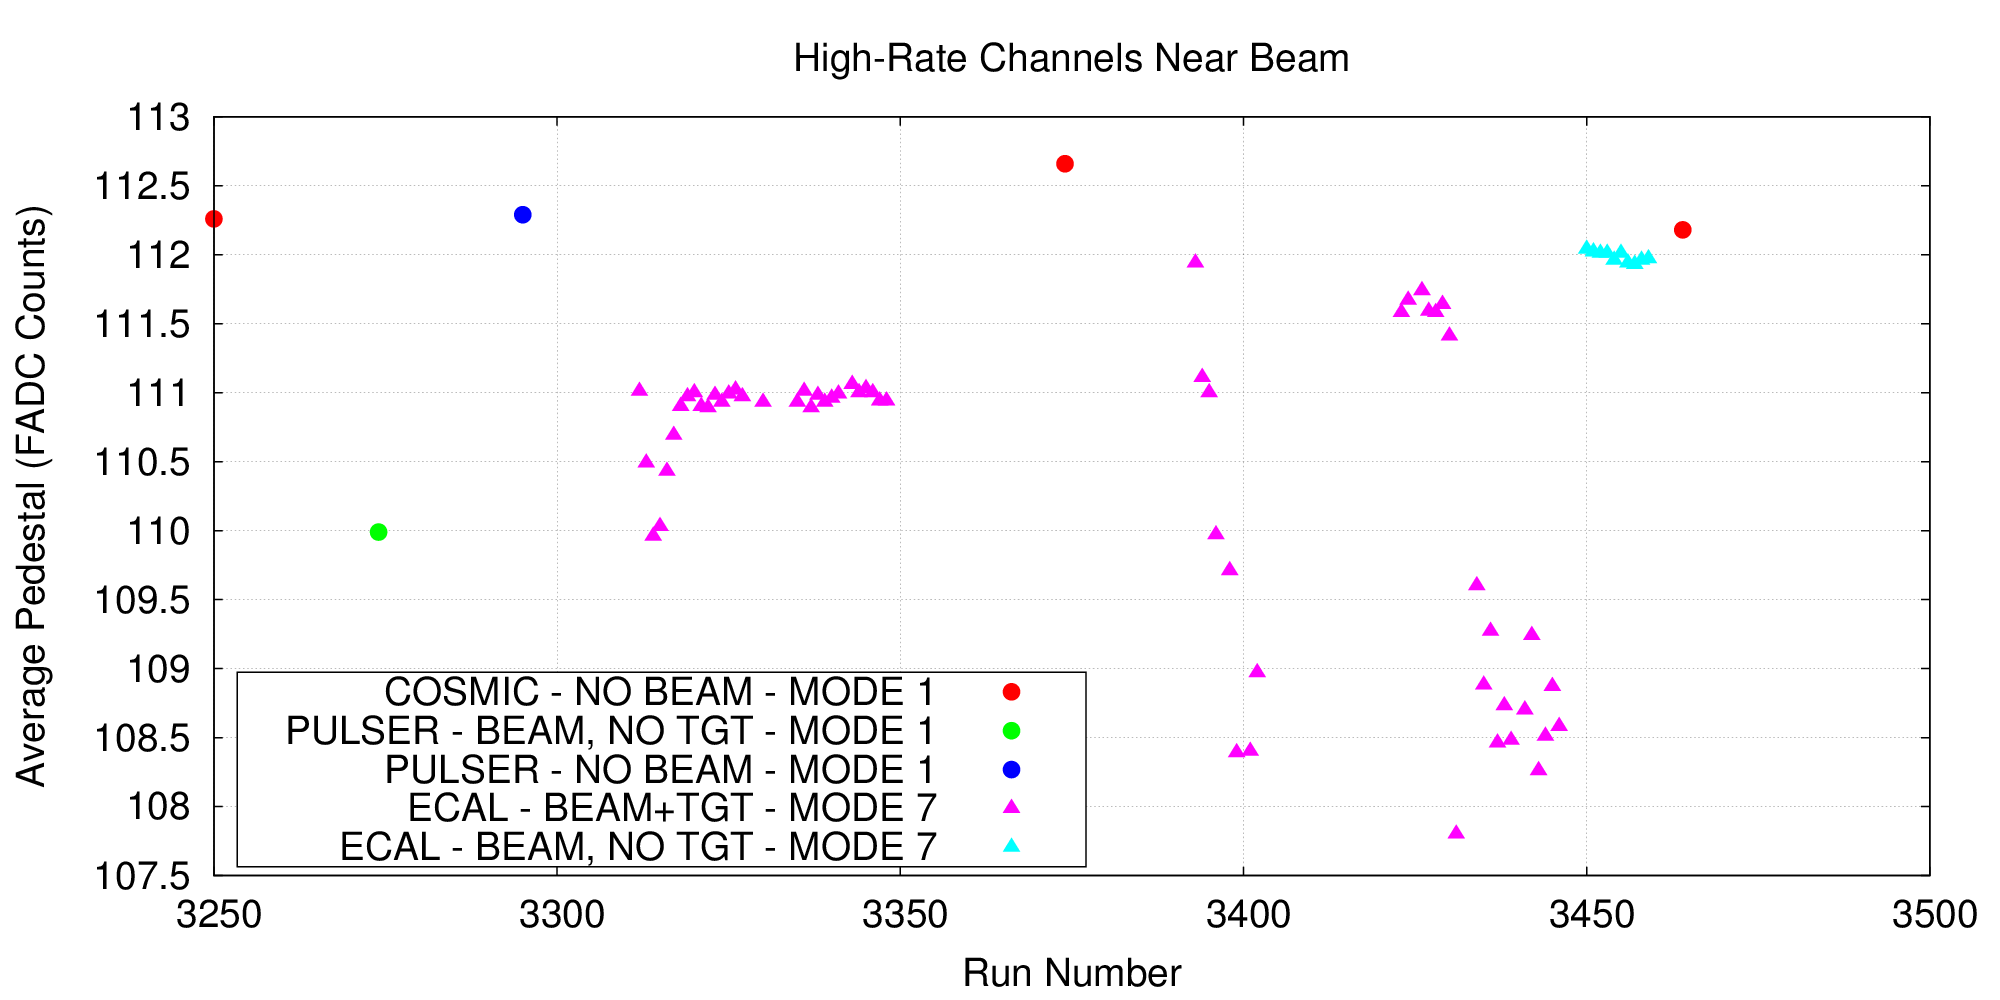
\includegraphics[width=14cm]{pics/hole.png}
    \caption{Run-dependence of pedestals, calculated with different methods and under different conditions, averaged over low- (top) and high- (bottom) rate channels.  The one point on the $y$-axis is actually from a much earlier run.  The green circle at run 3275 correponds to data with 150 nA beam current and {\em supposedly} no target.  The triangles cover a variety of currents, see Figure \ref{fig:pedvscur}. \label{fig:pedvsrun}}
\end{figure}
\newpage
\subsection{Discussion}
\begin{itemize}
\item
    The pedestals calculated from mode-1 and mode-7 with no beam/target basically agree in Figure \ref{fig:pedvsrun}.  Except for run 3275, a mode-1 run with pulser trigger, which could be explained by it really having a target in the beam in disagreement with the logbook.
    \item
        There is an obvious linear correlation between beam current and mode-7 pedestals for high-rate channels in Figure \ref{fig:pedvscur}.  From what I understand from Ben, this can be attributed to the capacitor in the calorimeter's APDs/preamps, causing the measured pedestals to decrease with pileup.  And, the measured effect appears to have an appropriate magnitude based on a rough estimate from our average rates and pulse energy.%  And it is well correlated with a channel's scaler's rate.
\item
The beam currents used for these plots are those recorded by the shift takers in the run spreadsheet.  The mode-7 pedestals are calculated from one file in each run.  The outliers from the nicely linear pedstal-current correlation could be  to incorrect beam current (from trips, human error, \ldots).
%An improvement could be to use the BPM currents recorded in the EPICS database.
\item
    For the most extreme channels with the highest rates, the pedestal decrease for 200 nA beam on 5 um Pt target is over 10 ADC, shown in Figure \ref{fig:pedvscur2}.  After inegrating the pulse and accounting for gains, this results in a 60 MeV underestimate of energy when using our current pedestals for those channels.  The effect roughly scales with rates in Figure \ref{fig:rates}.
\item
To deal with this in offline reconstruction:
\begin{itemize}
\item
For mode-7 data, we can use a running pedestal average from the data.
\item
For other modes, we can parameterize the pedestals as a function of current.
\end{itemize}
\item
This also means the threshold was effectively higher for high-rate channels.
\end{itemize}


\begin{figure}[htbp]\centering
    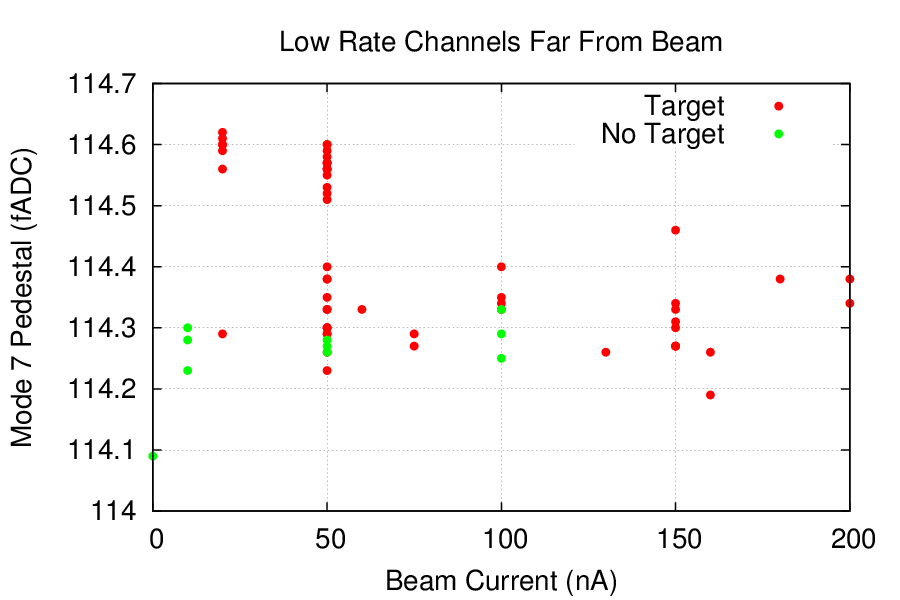
\includegraphics[width=8cm]{pics/ped_vs_current_low.png}
    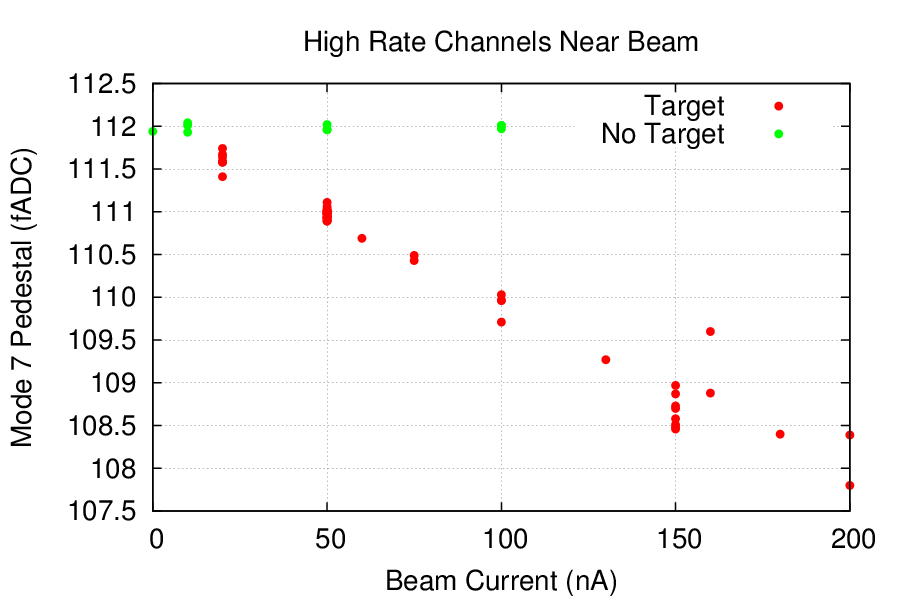
\includegraphics[width=8cm]{pics/ped_vs_current_high.png}
    \caption{Current-dependence of pedestals from FADC data recorded with mode-7, averaged over low-rate (left) and high-rate (right) channels.\label{fig:pedvscur}}
\end{figure}


\begin{figure}[htbp]\centering
    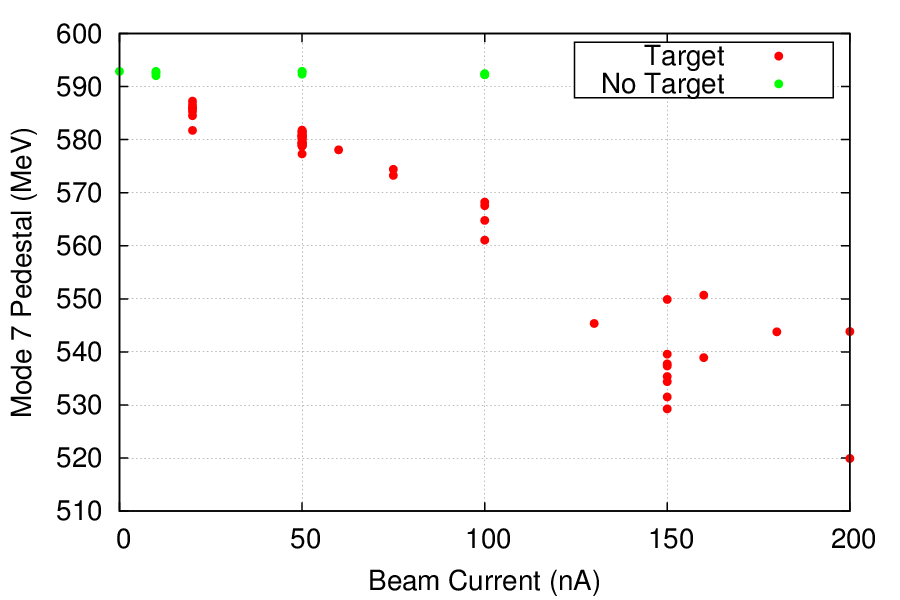
\includegraphics[width=8cm]{pics/pvsc_17_03_mev.png}
%    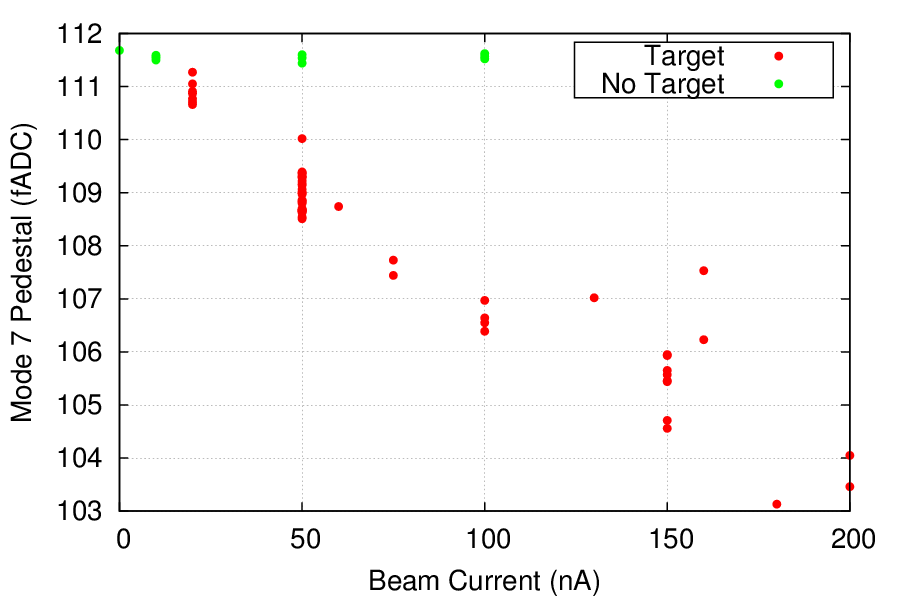
\includegraphics[width=8cm]{pics/pvsc_17_06.png}
    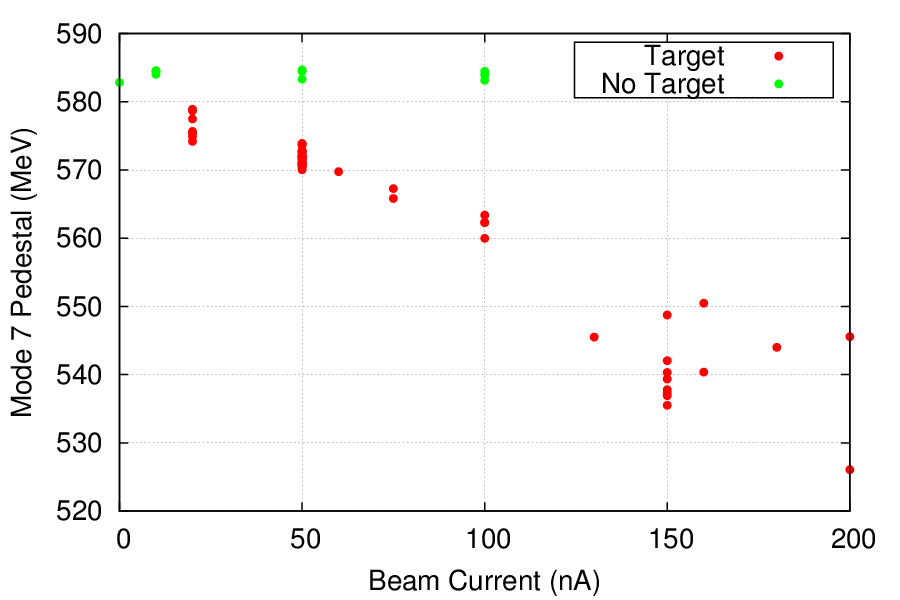
\includegraphics[width=8cm]{pics/pvsc_18_03_mev.png}
%    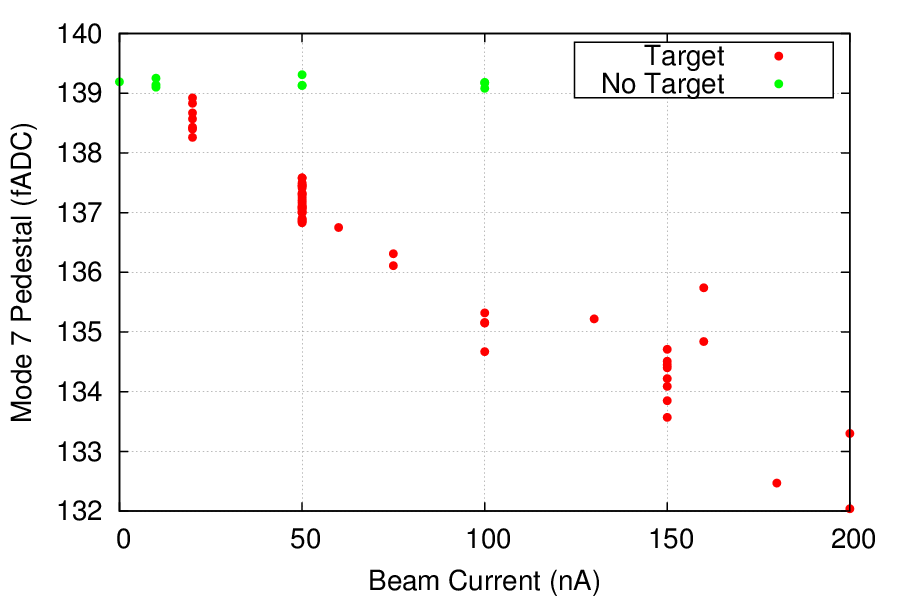
\includegraphics[width=8cm]{pics/pvsc_18_06.png}
    \caption{Current-dependence of pedestals for the two channels with the largest effect, $(x,y)$= $(-6,-2)$ and $(-5,-2)$, which are two of the channels with the highest rates (see Figure \ref{fig:rates}).  The $y$-axis is now the pedestal integrated over our pulse integration range and converted to energy by the average cosmic gain.\label{fig:pedvscur2}}
\end{figure}

\begin{figure}[htbp]\centering
    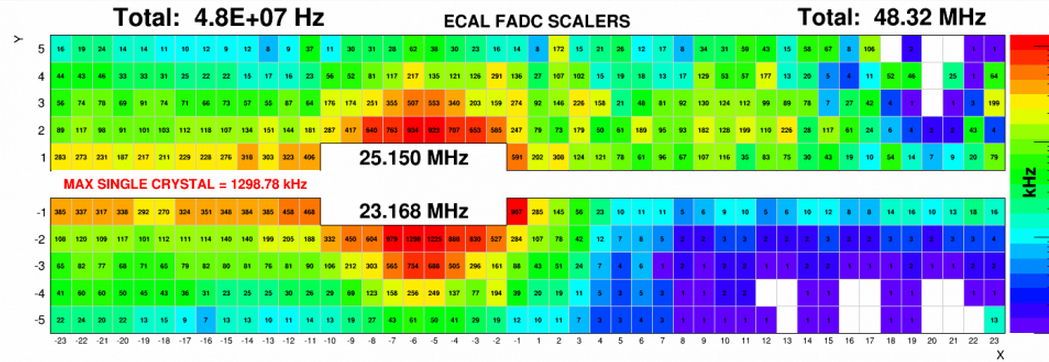
\includegraphics[width=17cm]{pics/rates.png}
    \caption{FADC scaler rates from run 3437 with 200 nA beam and 5 um Pt target.\label{fig:rates}}
\end{figure}

\begin{figure}[htbp]\centering
    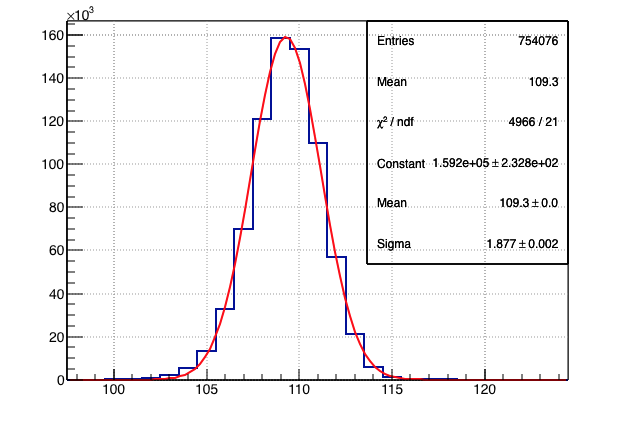
\includegraphics[width=8cm]{pics/20nA.png}
    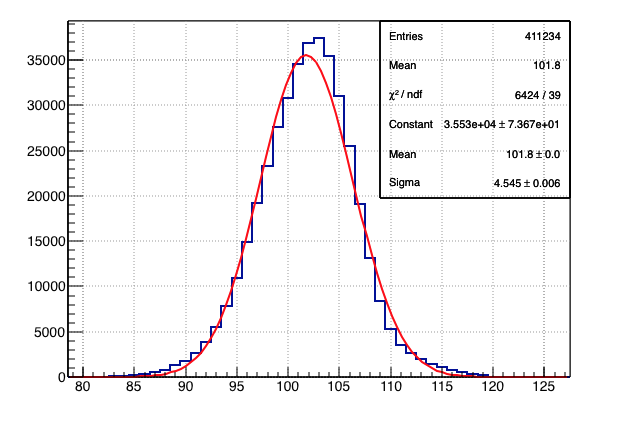
\includegraphics[width=8cm]{pics/200nA.png}
    \caption{Histograms of event-by-event 4-sample pedestals for a high-rate channel during 20 nA (left) and 200 nA (right) runs.  The broadening could be explained by the time-dependence in Figure \ref{fig:pedevt}.\label{fig:pedwidthhi}}
\end{figure}
\begin{figure}[htbp]\centering
    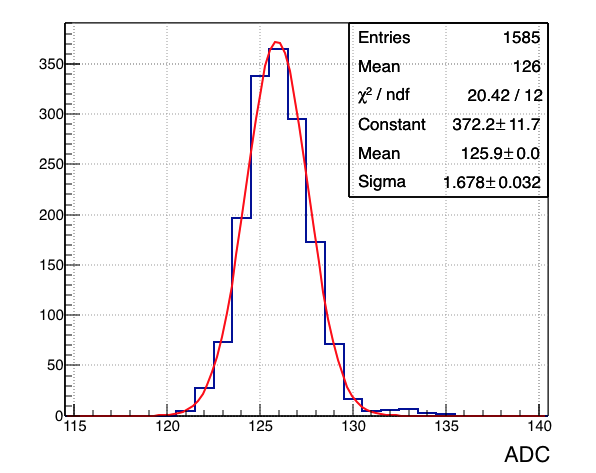
\includegraphics[width=8cm]{pics/20nA_00_00.png}
    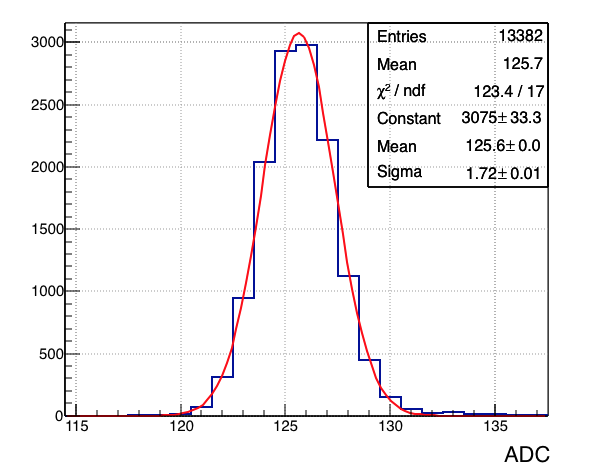
\includegraphics[width=8cm]{pics/200nA_00_00.png}
    \caption{Histograms of event-by-event 4-sample pedestals for a low-rate channel during 20 nA (left) and 200 nA (right) runs.  The lack of broadening is consistent with Figure \ref{fig:pedevt}.\label{fig:pedwidthlo}}
\end{figure}


\begin{figure}[htbp]\centering
    %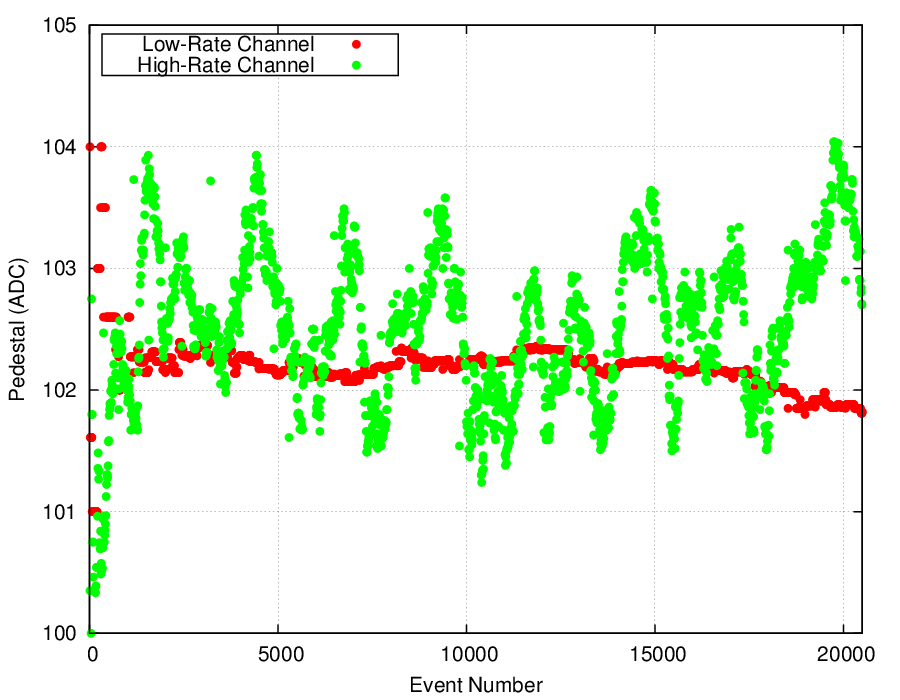
\includegraphics[width=12cm]{pics/pedevt.png}
    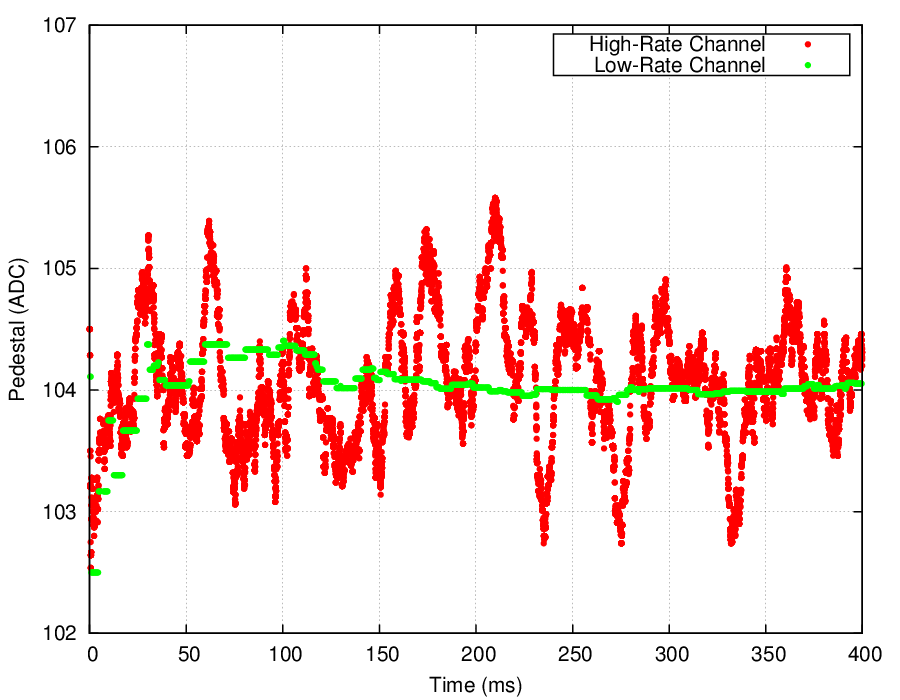
\includegraphics[width=12cm]{pics/3431_ped_vs_time4.png}
    \caption{A running pedestal average over the most recent 100 readouts of two channels in a 200 nA run.  The event rate was 60 kHz.  The spread at early times is while the average is still converging.  One issue with this is that we are reading the low-rate channel 100 times less frequently, and so possibly not sensitive to the effect in this plot.  However, since it's width is not increased as for the high rate channel in Figure \ref{fig:pedwidthlo}.
    \label{fig:pedevt}}
\end{figure}

\begin{figure}[htbp]\centering
    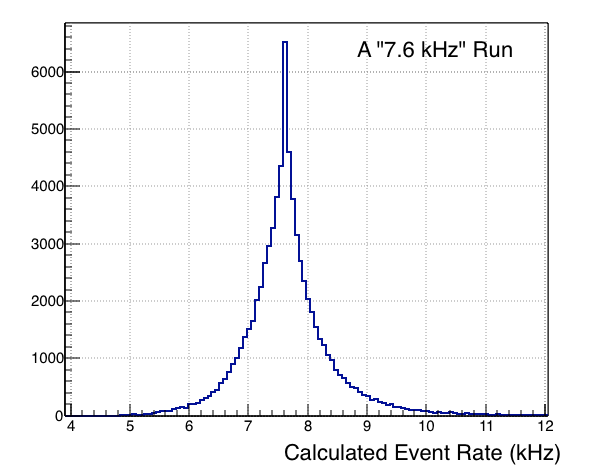
\includegraphics[width=12cm]{pics/7kHz.png}
    \caption{Event rate calculated from event time stamps for a run marked as ``7.6 kHz'' in the logbook. \label{fig:7.6}}
\end{figure}

\begin{figure}[htbp]\centering
    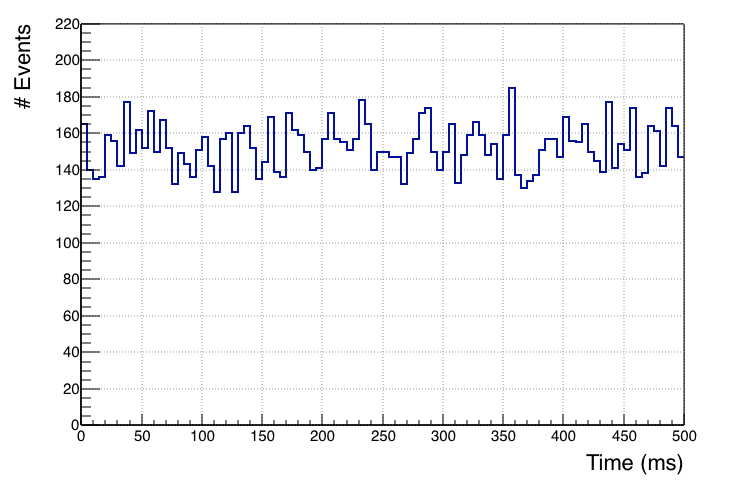
\includegraphics[width=12cm]{pics/nrate.png}
    \caption{Event rate as function of time.\label{fig:nrate}}
\end{figure}

%\section{Pileup Measurement}

%\bibliography{tpcalign}
\end{document}

